\documentclass[a4paper,11pt,headings=standardclasses,parskip=half]{scrartcl}

% font, style, etc.
\usepackage[utf8]{inputenc} % defines
\usepackage{csquotes}
\usepackage{xspace} % proper space after macros with 0 args
\usepackage{bm}

% mathematics
\usepackage{amsmath}
\usepackage{amssymb}

% figures, tables, etc.
\usepackage{hyperref} %
\usepackage{graphicx}
\usepackage{tikz}
\usepackage{pgf}
\usepackage{xcolor}
\usepackage{placeins} % -> floatbarrier
\usepackage{siunitx}  % -> handling of units

% code
\usepackage{listings}
\lstset{
language=Python, 
backgroundcolor = \color{light-gray},
basicstyle=\scriptsize\sffamily,
stringstyle=\color{orange},
breaklines=true,
numberstyle=\tiny\color{gray},
keywordstyle=\bfseries\color{dark-blue}\textit, % print keywords dark-blue
commentstyle=\color{dark-green}, % print comments dark-green
showstringspaces=false} % spacing between strings not showed

% t.b.d.
\newcommand{\listcode}[3]{\lstinputlisting[numbers=left,firstnumber=#1,firstline=#1,lastline=#2]{#3}}
\newcommand{\listcodeplanning}[2]{\listcode{#1}{#2}{../sim/01_trajectory_planning.py}}
\newcommand{\listcodecontrol}[2]{\listcode{#1}{#2}{../sim/02_car_example_control.py}}

% others
\usepackage{acronym}

% theorems
\newtheorem{defi}{Definition}[section]

% setup the appearance of links
\hypersetup{
    colorlinks = true, % false -> red box arround links (not very nice)
    linkcolor={blue!100!black},
    citecolor={blue!100!black},
    urlcolor={blue!100!black},
}

% manage glossaries
\usepackage{glossaries}
\makeglossaries
\newacronym{ivp}{IVP}{initial value problem}

% define shortcuts
\newcommand{\ad}{\mathrm{ad}}
\renewcommand{\d}{\mathrm{d}} % d vor differential forms
\newcommand{\NV}{{\cal N}\,}
\newcommand{\rang}{\mathrm{rang}}
\newcommand{\im}{\mathrm{im}}
\newcommand{\spann}{\mathrm{span}}
\newcommand{\R}{\mathbb{R}} %  set of real numbers
\newcommand{\py}{\emph{Python}\xspace}
\newcommand{\scipy}{\emph{SciPy}\xspace}
\newcommand{\mpl}{\emph{Matplotlib}\xspace}
\newcommand{\uu}{\mathbf{u}}
\newcommand{\x}{\mathbf{x}}
\newcommand{\y}{\mathbf{y}}
\newcommand{\z}{\mathbf{z}}
\newcommand{\xZero}{\mathbf{x}_0}

% color definitions
\definecolor{light-gray}{gray}{0.95}
\definecolor{dark-blue}{rgb}{0, 0, 0.5}
\definecolor{dark-red}{rgb}{0.5, 0, 0}
\definecolor{dark-green}{rgb}{0, 0.5, 0}
\definecolor{gray}{rgb}{0.5, 0.5, 0.5}

% ----------------------------------------------------------------------------
\subject{Control Theory Tutorial}% optional
\title{Car-Like Mobile Robot}
\subtitle{\py for trajectory planning and control}% optional
\author{}
\date{}
% ----------------------------------------------------------------------------


\begin{document}

\maketitle% create title

\tableofcontents

\newpage

\section{Introduction}
The goal of this tutorial is to teach the usage of the programming language \py as a tool for developing and simulating control systems. The following topics are covered:
\begin{itemize}
\item Implementation of different trajectory generators in a class hierarchy \py,
\item Flatness based feedforward control
\item Flatness based feedback control.

\end{itemize}
\textbf{\py source code file: \texttt{01\_trajectory\_planning.py}}

Later in this tutorial we will use the designed trajectory generators to design control strategies for the car model. 

Please refer to the \href{http://cs231n.github.io/python-numpy-tutorial/#python-containers}{Python List-Dictionary-Tuple tutorial} and the \href{http://cs231n.github.io/python-numpy-tutorial/#numpy}{NumPy Array tutorial} if you are not familiar with the handling of containers and arrays in Python. If you are completely new to \py consult the very basic introduction on \href{https://www.tutorialspoint.com/python/index.htm}{tutorialspoint}.
\section{Trajectories for smooth point-to-point transitions}
In control theory, we often want to transfer a system from a starting state $y(t_0)=y^A$ at the start time $t_0$ to a new state $y(t_f)=y^B$ at time $t_f$. The objective of smooth point-to-point transition is, that the generated trajectory $y_d: t \mapsto y$ meets certain boundary conditions at $t_0$ and $t_f$. If $y$ is for example a position coordinate and we use a simple trapezoidal interpolation in time between the two points $y^A$ and $y^B$, the amount of the acceleration at $t_0$ and $t_f$ approaches infinity which cannot be fullfilled by any system, due to inertia. That is why when we are planning a point-to-point transition we have to make sure, that the derivative of the planned trajectory is smooth up to a certain degree. 
\begin{figure}[ht]
\centering
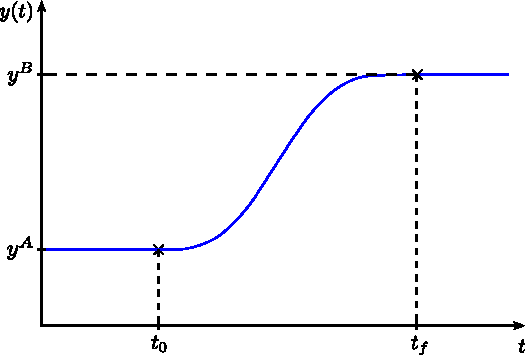
\includegraphics[scale=1]{img/state_transition.pdf}
\caption{Smooth state transition from $y^A$ to $y^B$}
\end{figure}
\subsection{Polynomials} \label{sec:polynomials}
A simple way of defining a trajectory between two points in time is a polynomial $y_d(t)=\sum_{i=0}^{2d+1}c_i\frac{t^i}{i!}$ of degree $2d+1$, where $2d+2$ is the number of boundary conditions it has to fulfill. We can write down $y_d(t)$ and its successive derivatives up to order $d$ in  matrix form:
\begin{align}
\label{eq:1}
\underbrace{\begin{pmatrix}
y_d(t) \\ \dot{y}_d(t) \\ \vdots \\ y_d^{(d-1)}(t) \\ y_d^{(d)}(t)
\end{pmatrix}}_{=:\mathbf{Y}_d(t) \in \R^{(d+1)}}
=\underbrace{\begin{pmatrix}
1 &t & \frac{t^2}{2!}&         &  \hdots         &  & \frac{t^{2d+1}}{(2d+1)!} \\
0 &1   & t             &         &  \hdots         &  & \frac{t^{2d}}{(2d)!} \\
0 &0   & 1               &         & \hdots          &  &  \frac{t^{2d-1}}{(2d-1)!} \\
\vdots &                 &  \ddots & \ddots &  &   &  \vdots \\
0      &\hdots           & \hdots       & 0 & 1& \hdots & \frac{t^{d}}{(d)!} \\
\end{pmatrix}}_{=:\mathbf{T}(t)\in \R^{(d+1)\times (2d+2)}}
\underbrace{
\begin{pmatrix}
c_0 \\ c_1 \\ \vdots \\ c_{2d-1}\\ c_{2d}\\ c_{2d+1} 
\end{pmatrix}}_{=:\mathbf{c}\in \R^{(2d+2)}}
\end{align}
To calculate the parameter vector $\mathbf{c}$, we first need to define the boundary conditions of the trajectory up to degree $d$:
\begin{align*}
\underbrace{\begin{pmatrix} y_d(t_0) \\ \dot{y}_d(t_0) \\ \vdots \\ y_d^{(d)}(t_0) \end{pmatrix}}_{:=\mathbf{Y}_d(t_0)}
&\overset{!}{=}
\underbrace{\begin{pmatrix} y^A \\ \dot{y}^A \\ \vdots \\ y^{(d)A}  \end{pmatrix}}_{:=\mathbf{Y}^A}
&&&
\underbrace{\begin{pmatrix} y_d(t_f) \\ \dot{y}_d(t_f) \\ \vdots \\ y_d^{(d)}(t_f) \end{pmatrix}}_{:=\mathbf{Y}_d(t_f)}
&\overset{!}{=}
\underbrace{\begin{pmatrix} y^B \\ \dot{y}^B \\ \vdots \\ y^{(d)B}  \end{pmatrix}}_{:=\mathbf{Y}^B}
\end{align*}
This leads to a linear equation system:
\begin{align*}
\begin{bmatrix}
\mathbf{Y}_d(t_0) \\
\mathbf{Y}_d(t_f) 
\end{bmatrix}
=
\begin{bmatrix}
\mathbf{Y}^A \\
\mathbf{Y}^B
\end{bmatrix}
&=
\begin{bmatrix}
\mathbf{T}(t_0) \\
\mathbf{T}(t_f) 
\end{bmatrix}
\mathbf{c}
\end{align*}
Because $\begin{bmatrix}
\mathbf{T}(t_0) \\
\mathbf{T}(t_f) 
\end{bmatrix}$ is quadratic and not singular for $t_0,t_f\neq 0$, we can solve this linear equation system explicitly:
\begin{align}
\label{eq:2}
\mathbf{c} &= \begin{bmatrix}
\mathbf{T}(t_0) \\
\mathbf{T}(t_f) 
\end{bmatrix}^{-1}
\begin{bmatrix}
\mathbf{Y}^A \\
\mathbf{Y}^B
\end{bmatrix}
\end{align}
Because the calculation of the invertible matrix is computationally expensive, in an implementation, it is more efficient to use a linear equation system solver, like \texttt{linalg.solve()} from \emph{Numpy}, to solve for $\mathbf{c}$

Now we can calculate $\mathbf{Y}(t)$ in a closed form:
\begin{align}
\label{eq:3}
\mathbf{Y}(t)=\mathbf{T}(t)\mathbf{c} \quad t \in [t_0,t_f] 
\end{align}
The full trajectory can be defined as a piecewise function:
\begin{align}
y(t)=\begin{cases}y^A & \textrm{if } t<t_0 \\ y_d(t) =\sum_{i=0}^{2d+1}c_i\frac{t^i}{i!} & \textrm{if } t\in [t_0,t_f] \\y^B & \textrm{if } t>t_f\end{cases}
\end{align}
\subsection{Implementation in \py}
In order to automate the process of trajectory planning we first create a \emph{Planner} base class. Then we create a new subclass for each new planning algorithm, we want to use.
\subsubsection{The \emph{Planner} base class}
A \emph{Planner} should have the following attributes:
\begin{itemize}
	\item[] \texttt{YA} - vector of $y$ and it's derivatives up to order \texttt{d} at start time \texttt{t0}
	\item[] \texttt{YB} - vector of $y$ and it's derivatives up to order \texttt{d} at final time \texttt{tf}
	\item[] \texttt{t0} - start time of the point-to-point transition
	\item[] \texttt{tf} - final time of the point-to-point transition
	\item[] \texttt{d} - planned trajectory should be smooth up to the $d$-th derivative
\end{itemize}
We also want to evaluate the planned trajectory, but how this is done should be implemented in the specific subclass. By using in abstract base class method, we force a subclass of \emph{Planner} to have a method \texttt{eval()}.
\listcodeplanning{2}{27}
\subsubsection{The \emph{PolynomialPlanner} subclass}
To implement the planning algorithm that was developed in \autoref{sec:polynomials}, we create a new class \texttt{PolynomialPlanner} that inherits from the previously defined class \texttt{Planner}. All the attributes and methods of \texttt{Planner} are now also attributes and methods of \texttt{PolynomialPlanner}.
\listcodeplanning{30}{35}
To solve for the parameter vector $\mathbf{c}$, we have to calculate the matrix $\mathbf{T}(t)$ from \eqref{eq:1}. We therefore create a method \texttt{TMatrix()}:
\listcodeplanning{75}{96}
Now we we have to create a method, that solves \eqref{eq:2} and returns $\mathbf{c}$:
\listcodeplanning{99}{118}
Because we want to reuse the result, we create a new attribute \texttt{c}:
\listcodeplanning{37}{39}
Finally we define a method \texttt{eval()} that implements \eqref{eq:3}:
\listcodeplanning{41}{56}
as well as a second method \texttt{eval\_vec()}, that can handle a time array as an input:
\listcodeplanning{59}{72}
The polynomial trajectory planner is now implemented and can be tested.

\textbf{Example:}
Suppose we want to plan a trajectory from $y(t_0)=0$ to $y(t_f) = 1$ with $t_0=1s$ and $t_f = 2s$. The trajectory should be one time smooth differentiable $(d=1)$. We therefore have to define the boundary conditions for the first derivative of $y$: 
\begin{align*}
\dot{y}(t_0)=0 &&& \dot{y}(t_f)=0
\end{align*}
The total time interval for the evaluation of the trajectory is $t\in[0s,3s]$.

In \py we first define the boundary conditions for $t=t_0$ and $t=t_f$:
\listcodeplanning{122}{123}
Then we define the start and final time of the transition and the total time interval:
\listcodeplanning{124}{126}
Then we set $d$ and create a \texttt{PolynomialPlanner} instance \texttt{yd} with the defined parameters.
\listcodeplanning{127}{128}
We can display the calculated parameters
\listcodeplanning{130}{131}
and sample the generated trajectory at the defined total time interval
\listcodeplanning{133}{134}
At last, we can plot the results
\listcodeplanning{136}{142}
\begin{figure}[ht]
\centering
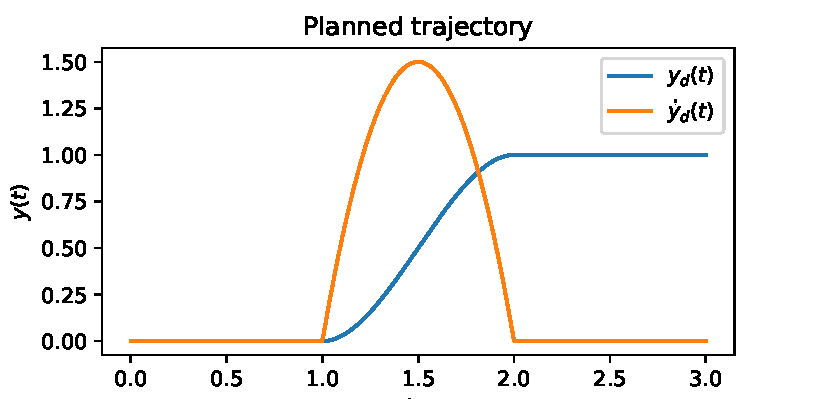
\includegraphics[scale=1]{img/planned_trajectory.pdf}
\end{figure}

\newpage
\section{Feedforward control for the car}
\printglossaries
\end{document}

%%% Local Variables:
%%% mode: latex
%%% TeX-master: t
%%% End:
